\begin{frame}
  {\texttt{\$ who}}

  \begin{columns}
    \begin{column}{0.48\textwidth}
      {\texttt{@f0rki}}
      \begin{itemize}
        \item f0rki@hack.more.systems
        \item CS/InfoSec Student
        \item CTF Player since 2010
      \end{itemize}
    \end{column}

    \begin{column}{0.48\textwidth}
      \texttt{@stefan2904}
      \begin{itemize}
        \item stefan@hack.more.systems
        \item CS/InfoSec/CI Student
        \item CTF Player since 2014
      \end{itemize}
    \end{column}
  \end{columns}

\end{frame}


\begin{frame}{stuff we are gonna be talking about \ldots}
    \tableofcontents
\end{frame}


\section{Introduction to CTFs}

\begin{frame}[fragile]
  {CTF: Capture The Flag}

  \begin{itemize}
    \item Collaborative hacking competitions
    \begin{itemize}
    	\item Teams vs. Teams
    \end{itemize}
    \item The goal is to capture Flags
  \end{itemize}
\end{frame}



\begin{frame}[fragile]{}
	 \begin{center}
	 	\Huge\verb+CTF{THIS_IS_A_FLAG}+
	 \end{center}
\end{frame}

\begin{frame}
  {CTF Type: Jeopardy}

  \begin{center}
    %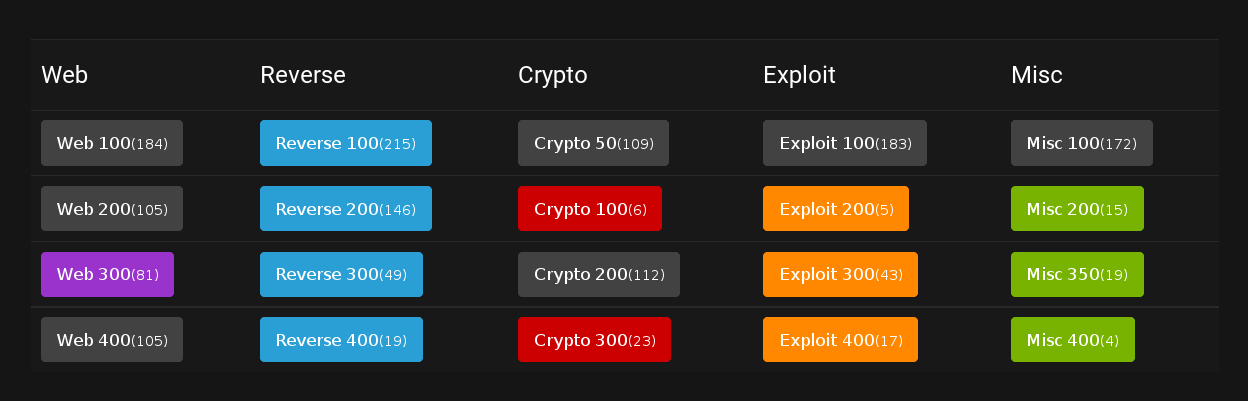
\includegraphics[width=\textwidth]{./images/dctf-challenges.png}
    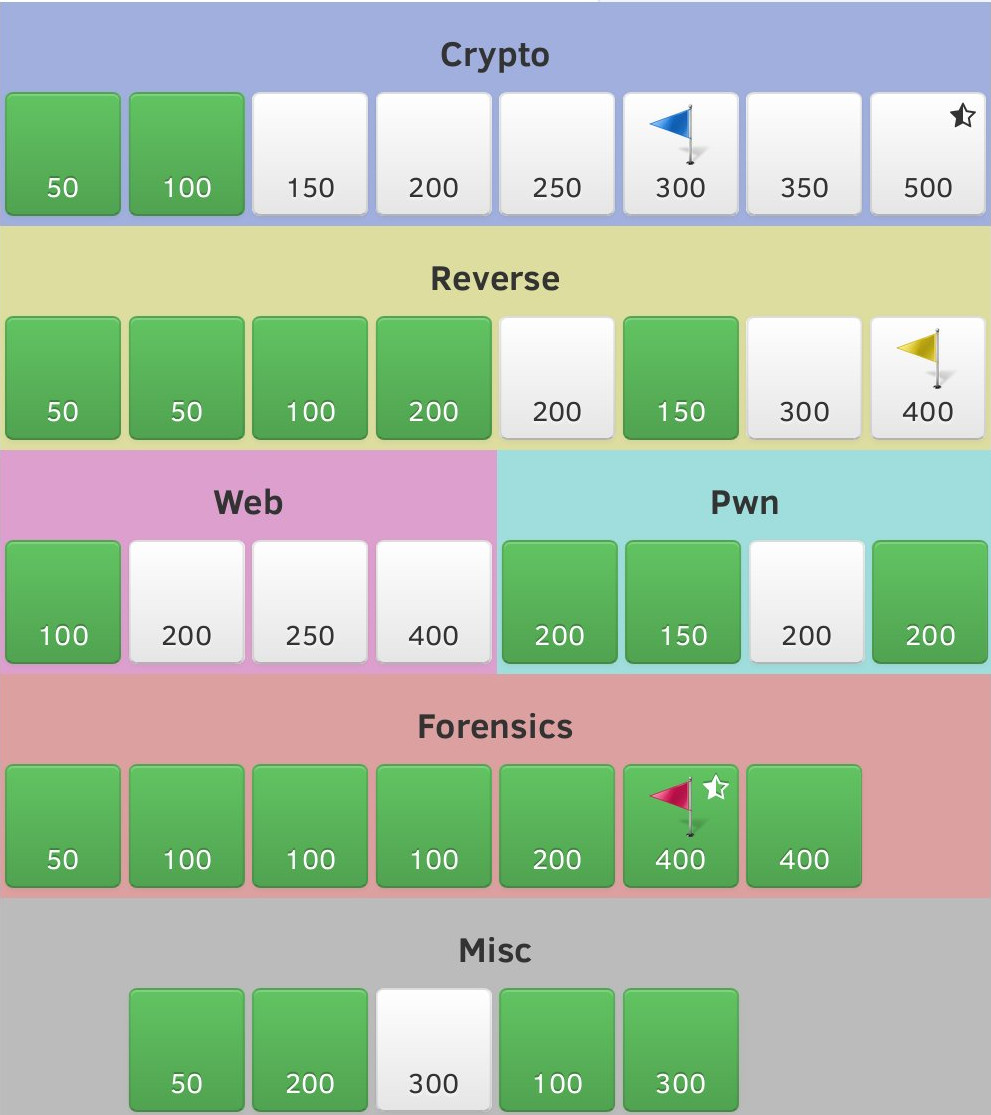
\includegraphics[height=0.8\textheight]{./images/sharifctf-challenges.jpg}
  \end{center}
\end{frame}

\begin{frame}
  {CTF Type: Attack-Defense}

  \begin{figure}[h]
    \centering
    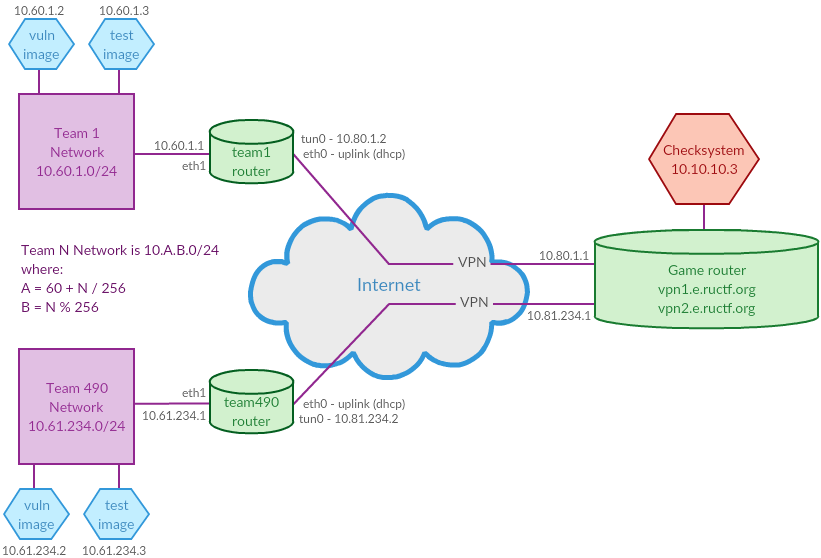
\includegraphics[width=0.9\textwidth]{./images/ructf-network.png}
    \caption{RUCTFe 2015 Network Schema (source:
      \href{https://ructf.org/e/2015/network.html}{RUCTF org}) }
  \end{figure}
\end{frame}

\begin{frame}
  {CTF Type: Attack-Defense}

  \begin{figure}[h]
    \centering
    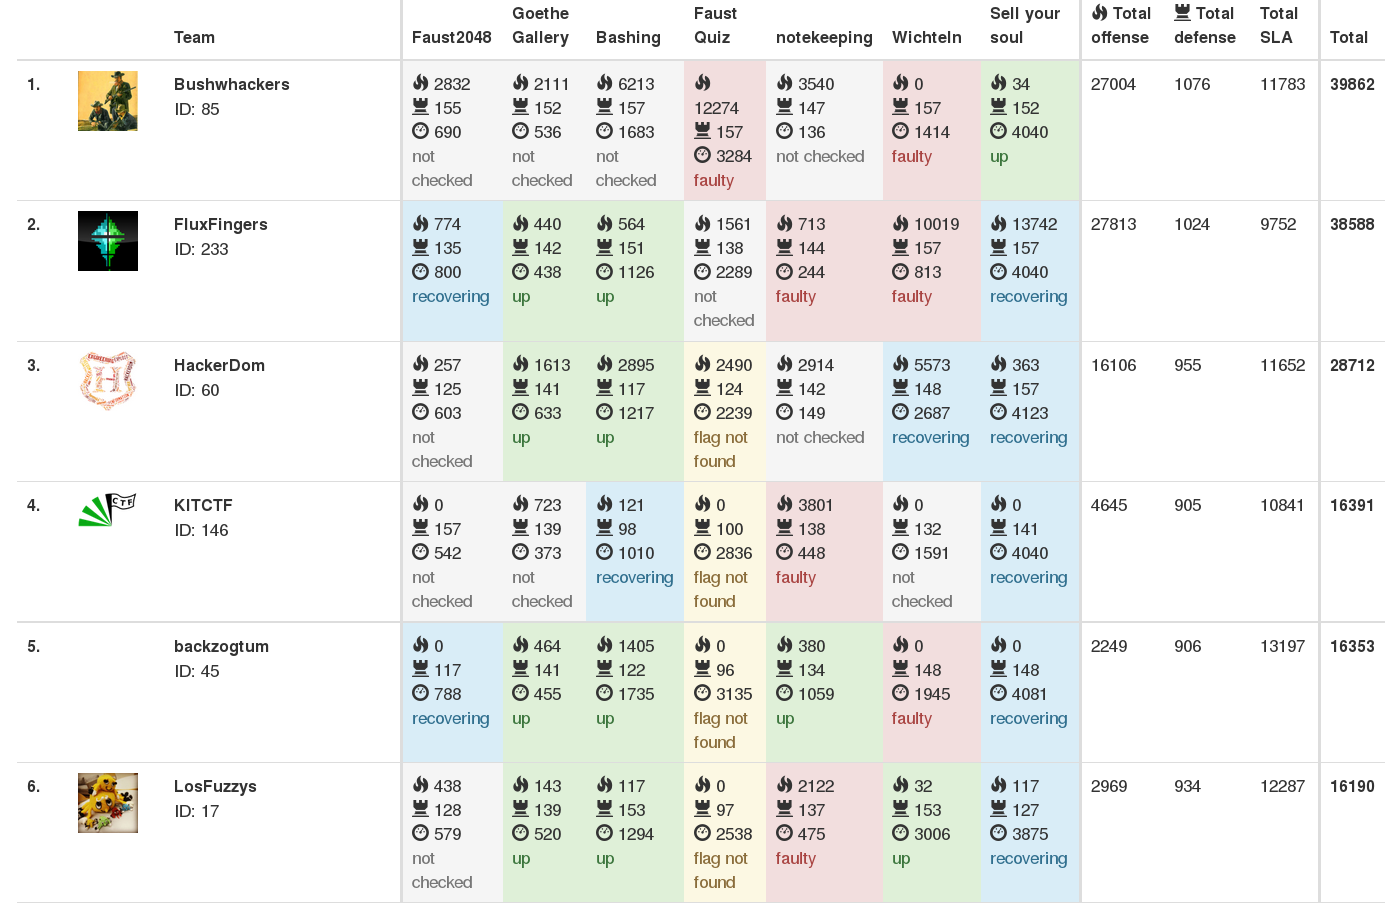
\includegraphics[width=\textwidth]{./images/faustctf-scoreboard.png}
    \caption{FAUST CTF 2015 scoreboard}
    \label{fig:faustctfscoreboard}
  \end{figure}

\end{frame}


\begin{frame}
  {Why CTFs?}

  \begin{itemize}
    \item \textbf{It's fun!}
    \item Gain experience in InfoSec
    \item Challenges modeled after real-world problems
      \begin{itemize}
        \item Sometimes real-world bugs modeled after CTF bugs?
      \end{itemize}
  \end{itemize}
\end{frame}

\section{LosFuzzys}

\begin{frame}[allowframebreaks]
  {\texttt{LosFuzzys}: A CTF Team in Graz}
  {We Like Bugs!}

  \begin{figure}[H]
    \centering
    \includegraphics[height=0.7\textheight]{images/zippy/zippy_family2.jpg}
  \end{figure}

  \framebreak

  \begin{itemize}
    \item \url{https://hack.more.systems}
      \\ twitter: \href{https://twitter.com/LosFuzzys}{@LosFuzzys}
    \item A group of people interested in information security
    \item Primarily CS/SW/ICE Students from TUGraz
      \begin{itemize}
        \item But we welcome anyone interested and motivated :)
        \item and maybe even you ;)
      \end{itemize}
    \item Irregular Meet-ups
  \end{itemize}
\end{frame}

\begin{frame}
	{Where to start?}

	\begin{itemize}
		\item Talk to us! :-)
	\end{itemize}

	\begin{itemize}
		\item Read writeups!
		\begin{itemize}
			\item Repo: \href{https://github.com/ctfs}{github.com/ctfs}
			\item Ours: \href{https://hack.more.systems/writeups}{hack.more.systems/writeups}
		\end{itemize}
	\end{itemize}

\end{frame}

\section{CTF Toolbox}

\begin{frame}
  {CTF Hackers Toolbox}

  \begin{itemize}
    \item Great diversity of challenges
    \item Some things turn up frequently
    \item Knowledge of technology necessary
    \item Experience helps a lot
  \end{itemize}

  \begin{itemize}
    \item Using the right tools is essential
      \begin{itemize}
        \item assuming you know how to use them\ldots
      \end{itemize}
  \end{itemize}

\end{frame}

\begin{frame}
  {Scripting is your best Friend}

  \begin{itemize}
    \item Python, Ruby, Bash etc.
    \item Be comfortable in one of those
  \end{itemize}

  \begin{center}
    
\includegraphics[height=0.5\textheight]{images/automatealltheexploits.jpg}
  \end{center}
\end{frame}


\begin{frame}
  {Command-Line-Fu is very helpful}

  \begin{itemize}
    \item Network stuff -- \texttt{nc, socat, dig, nmap}
    \item Query json files -- \texttt{jq}
    \item HTTP -- \texttt{curl}
  \end{itemize}

  \begin{itemize}
    \item Chain together to get your results!
  \end{itemize}
\end{frame}


\begin{frame}
  \todo[inline]{add command line black-magic example}
\end{frame}

% python requests - automated browsing

\begin{frame}[fragile]
  {Automated Browsing -- python-requests}

  \begin{lstlisting}[language=python]
import requests

URL = 'http://ctf.example.com'
s = requests.session()
r = s.post(URL + '/login',
           data={'user': 'fuzzy', 'pass': '1234'})

# GET http://ctf.example.com/vuln?x='or%201=1--x
resp = s.get(URL + '/vuln',
             params={'x': '\'or 1=1 --x'})
# session cookie automagically used here

print resp.text
# flag{some_flag_of_some_service}
  \end{lstlisting}
\end{frame}

% pwntools - implement parts of line-based network protocols

\begin{frame}[fragile]
  {dirty networking -- pwntools/binjitsu}

% TODO: send email or something
  \begin{lstlisting}[language=python]
from pwn import *

r = remote('ctf.example.com', 1337)

# line based
r.recvline()
r.sendline('HELO %s%s%s%s')
r.recvuntil('250 Hello')

data = r.recv(4)

# unpack LE uint32 from bin
i = u32(data)
log.info('received uint32 {}'.format(i))

# pack BE uint32 to bin
r.send(p32(1094795585, endian='big'))
r.recvline()
  \end{lstlisting}
\end{frame}


\begin{frame}[fragile]


  {\Huge A wild binary appears!}

  \begin{lstlisting}
$ file ./pwn
pwn: ELF 32-bit LSB executable, Intel 80386,
  version 1 (GNU/Linux), statically linked,
  for GNU/Linux 2.6.24,
  not stripped
  \end{lstlisting}
\end{frame}


\begin{frame}[fragile]
  \begin{center}
    \verb+$ objdump -d pwn | less+

    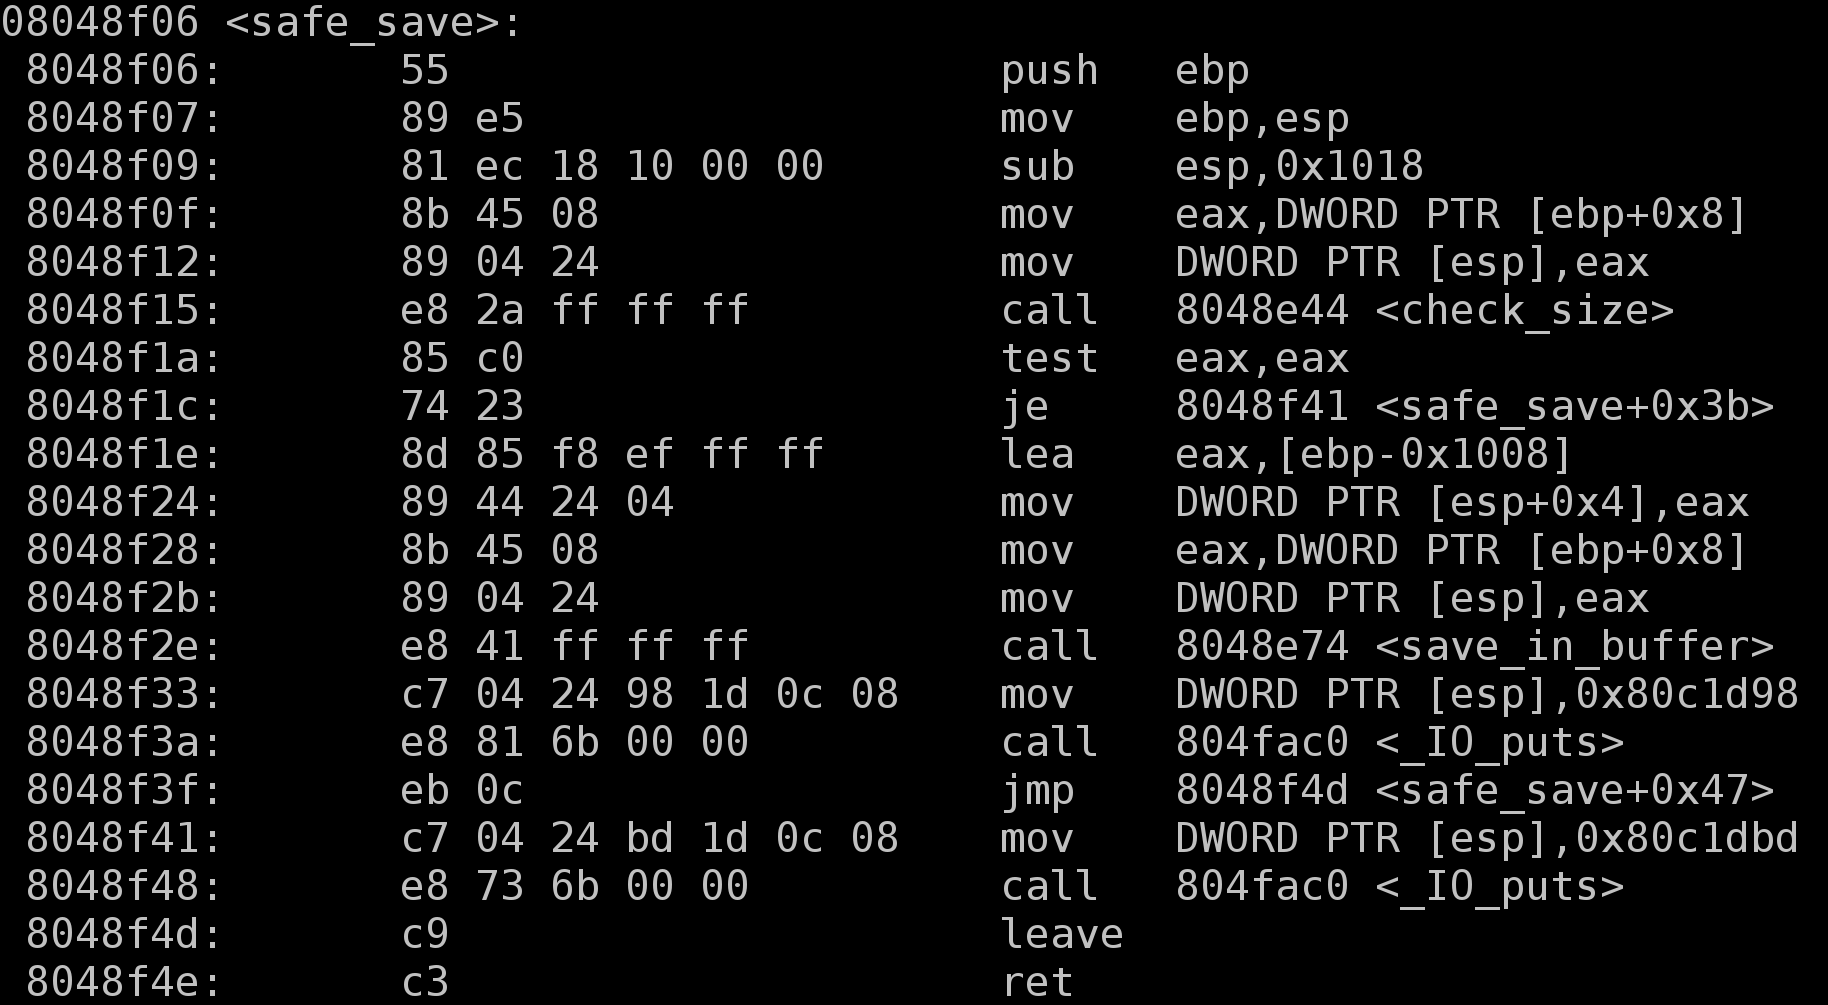
\includegraphics[width=0.95\textwidth]{./images/objdump.png}
  \end{center}
\end{frame}


\begin{frame}
  {radare2 to the rescue}
  \begin{center}
    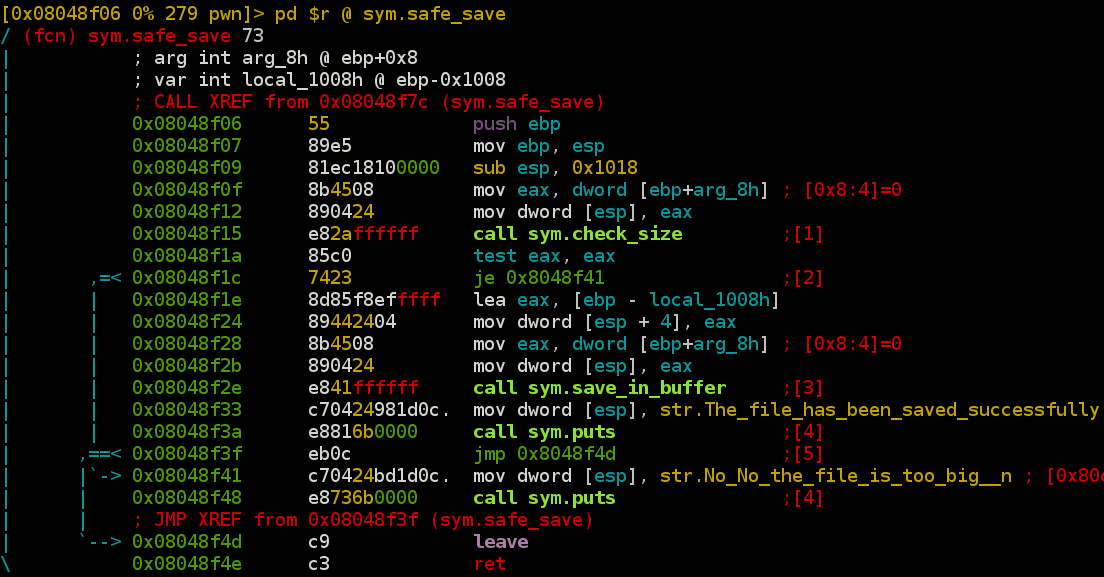
\includegraphics[width=\textwidth]{./images/radare-disas.png}
  \end{center}
\end{frame}

\begin{frame}
  \begin{center}
    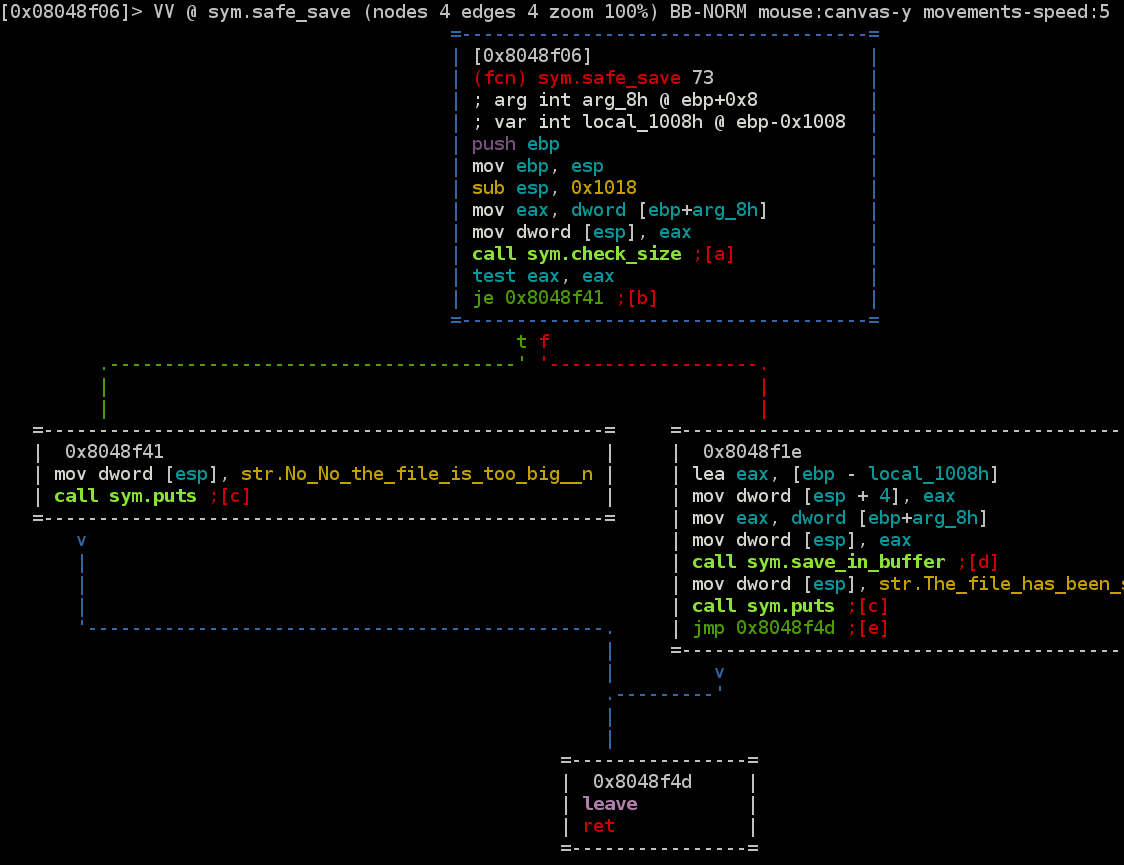
\includegraphics[width=\textwidth]{./images/radare-disas2.png}
  \end{center}
\end{frame}

\begin{frame}
  \begin{center}
    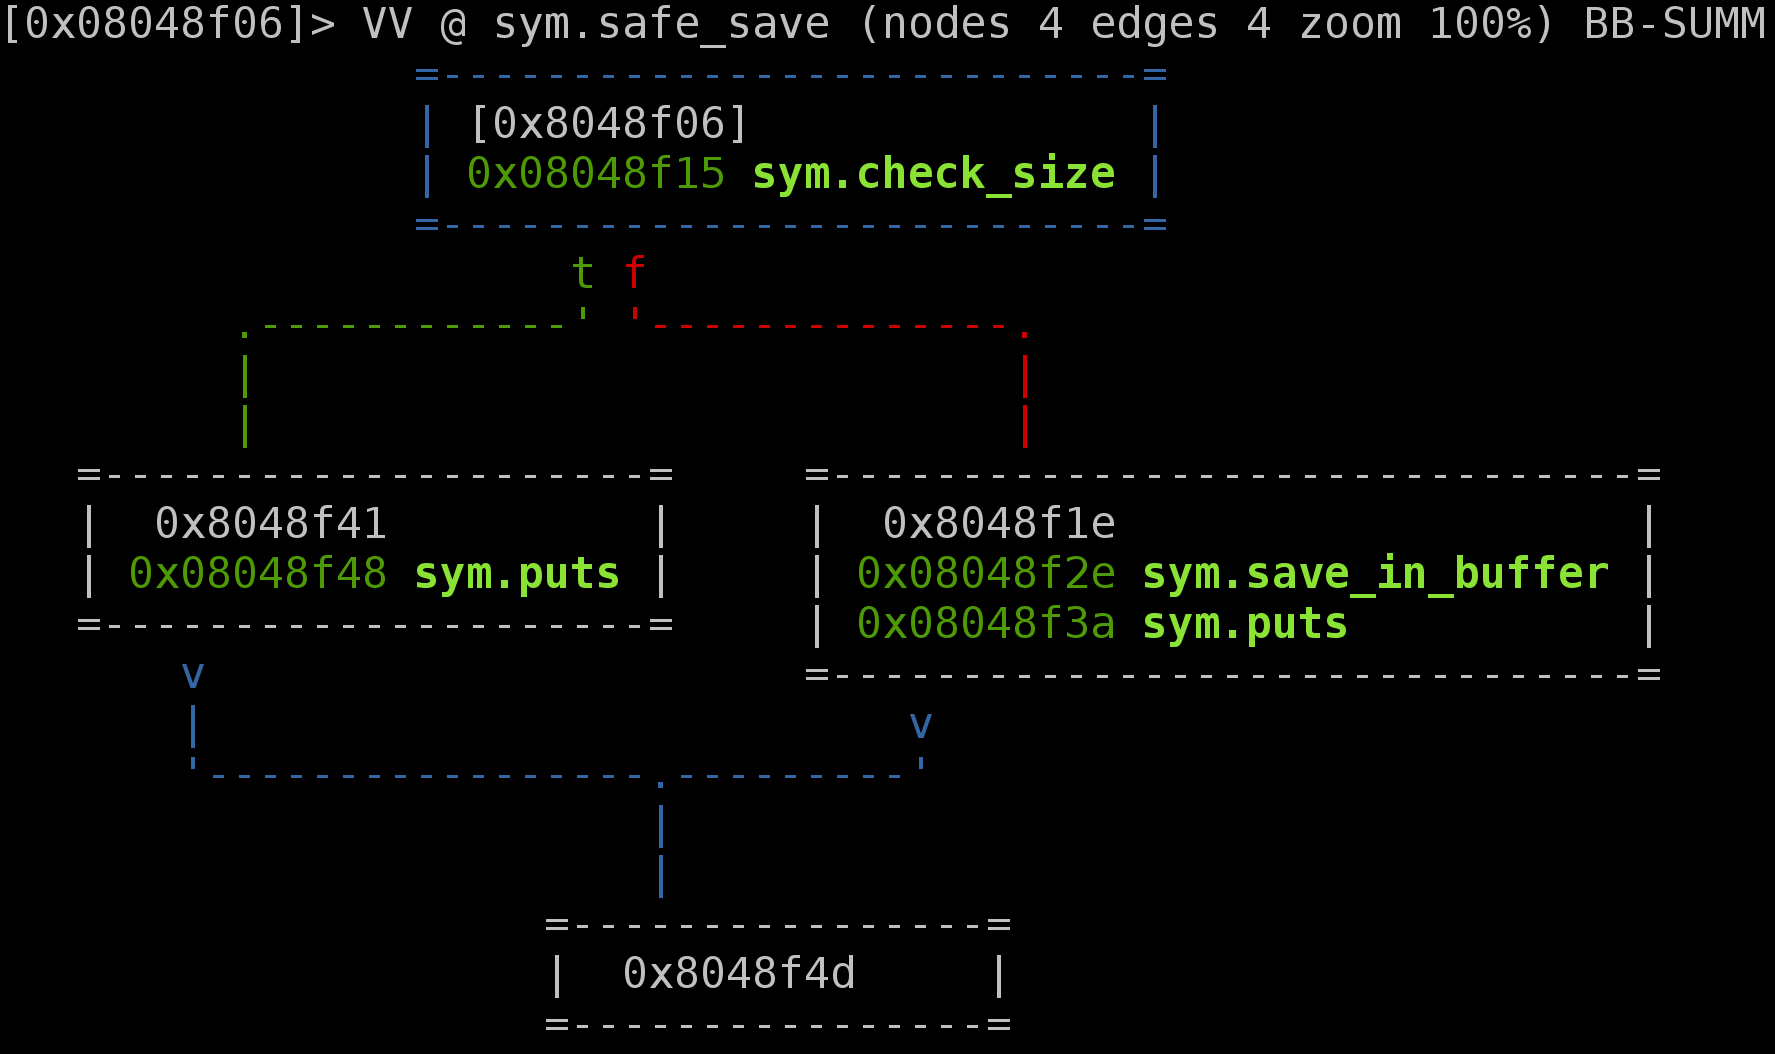
\includegraphics[width=\textwidth]{./images/radare-disas3.png}
  \end{center}
\end{frame}

\begin{frame}
  {radare2 -- reversing tool}

  \begin{itemize}
    \item Disassembler/Assembler
    \item Debugger
    \item Code emulator
    \item Hex Editor
    \item \ldots
  \end{itemize}
\end{frame}

% gdb - pretty horrible

\begin{frame}
	\begin{center}
    \huge Debugging?
	\end{center}
\end{frame}

\begin{frame}
  \begin{center}
    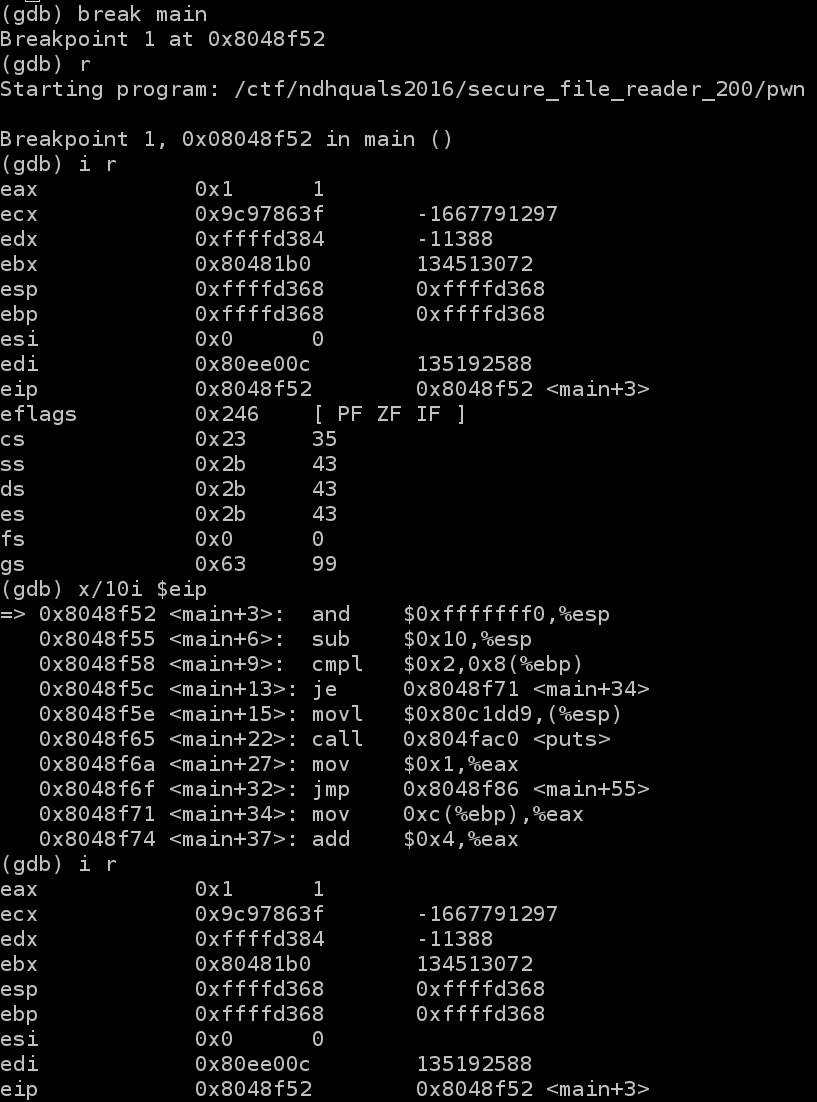
\includegraphics[width=0.8\textwidth]{./images/gdb-plain.png}
  \end{center}
\end{frame}

\begin{frame}
  \begin{center}
    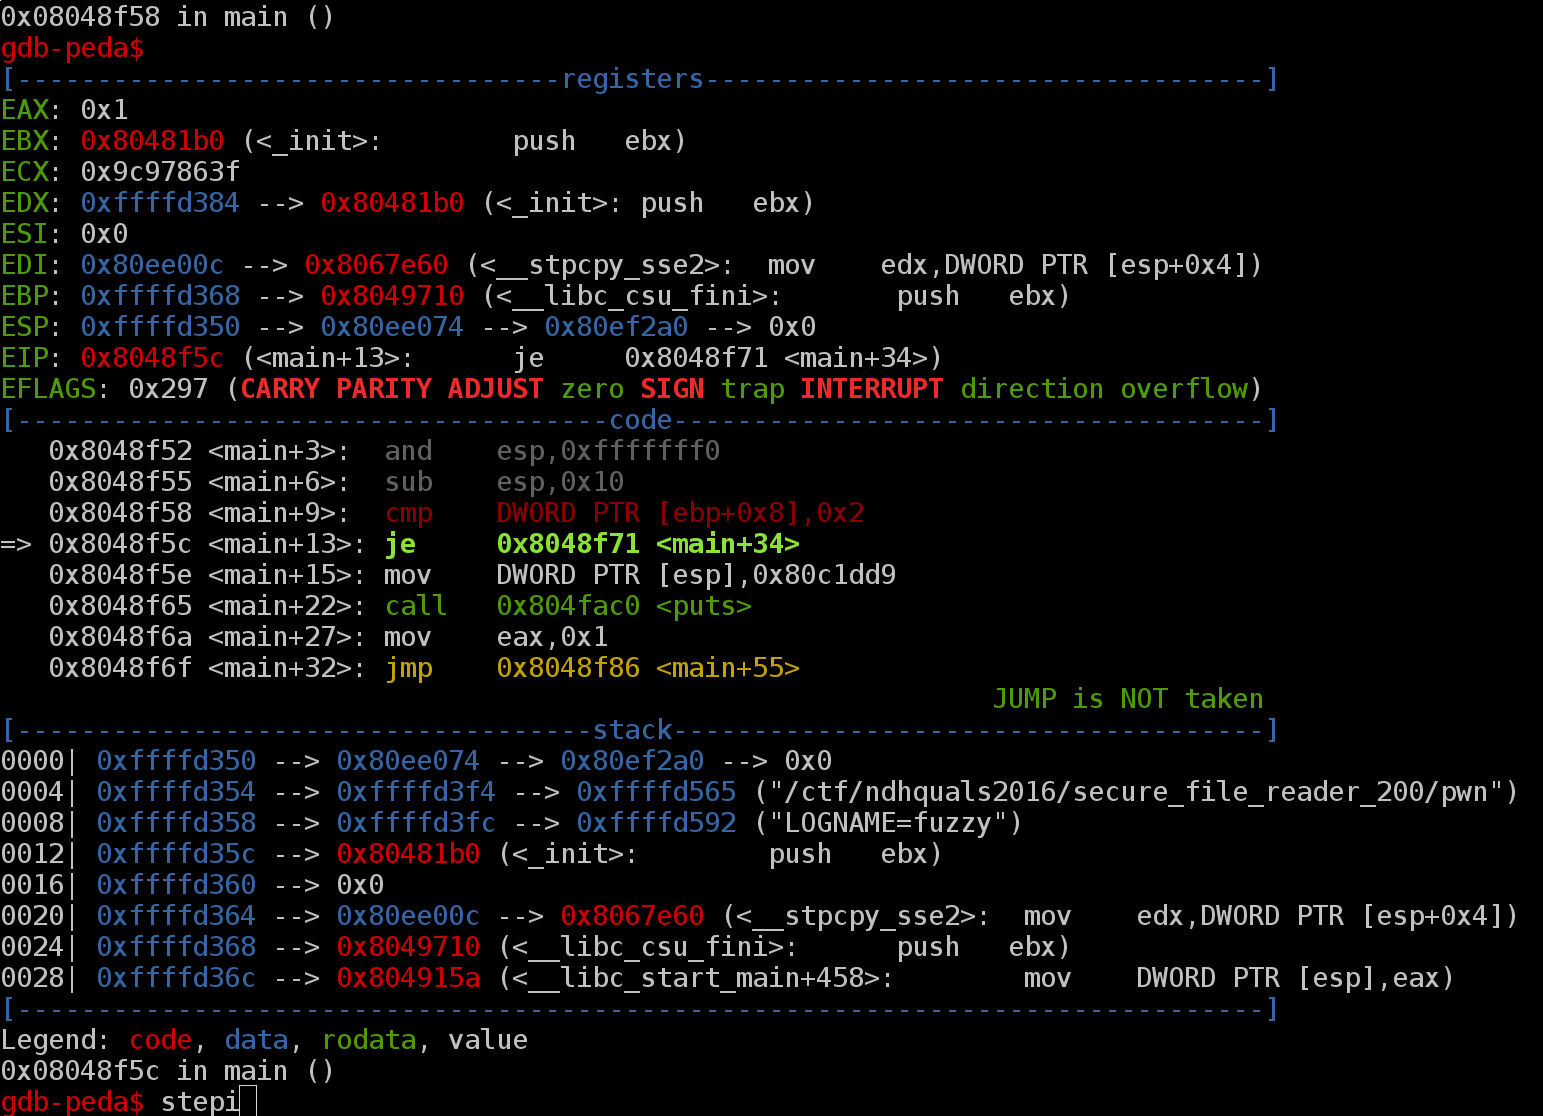
\includegraphics[width=\textwidth]{./images/gdb-peda.png}
  \end{center}
\end{frame}

\begin{frame}
  {Debuggers}

  \begin{itemize}
    \item Use gdb with one of those:
      \begin{itemize}
        \item \href{https://github.com/longld/peda}{PEDA}
        \item \href{https://github.com/hugsy/gef}{GEF}
        \item \href{https://github.com/zachriggle/pwndbg}{pwndbg}
        \item \href{https://github.com/snare/voltron}{voltron}
        \item \href{https://github.com/cyrus-and/gdb-dashboard}{gdb-dashboard}
      \end{itemize}
    \item gdb alternatives: lldb, radare2
    \item Newer debugging approaches
      \begin{itemize}
        \item \href{https://github.com/BinaryAnalysisPlatform/qira}{qira}
        \item \href{http://rr-project.org/}{rr}
      \end{itemize}
  \end{itemize}
\end{frame}


\begin{frame}
  {QIRA -- ``Timeless Debugging''}

  \todo[inline]{add qira screenshot}

\end{frame}


% pwntools - build exploits and pwn binaries

\begin{frame}[fragile]

  {\Huge Pwning!}

  \begin{lstlisting}
$ mkfifo fifo
$ ./pwn fifo & python -c 'print("A"*4128)' >> fifo
[1] 9391
The file has been saved successfully
[1]  + 9391 segmentation fault (core dumped)  ./pwn fifo
$ dmesg | tail -n 1
pwn[9391]: segfault at 41414141 ip 0000000041414141
  sp 00000000ffb6d340 error 14
  \end{lstlisting}
\end{frame}


\begin{frame}[fragile]
  {pwntools again!}

  \begin{lstlisting}[language=python]
from pwn import *  # NOQA
import subprocess

velf = ELF("./pwn")
r = ROP(velf)
r.call("exit", [42])
payload = "A" * 4124 + str(r)

# launch process
vp = process(["./pwn", "./fifo"])
# gdb.attach(vp)
# break *0x8048f4e

with open("./fifo", "w") as f:
    f.write(payload)

vp.interactive()
  \end{lstlisting}
\end{frame}

\begin{frame}
  \begin{center}
    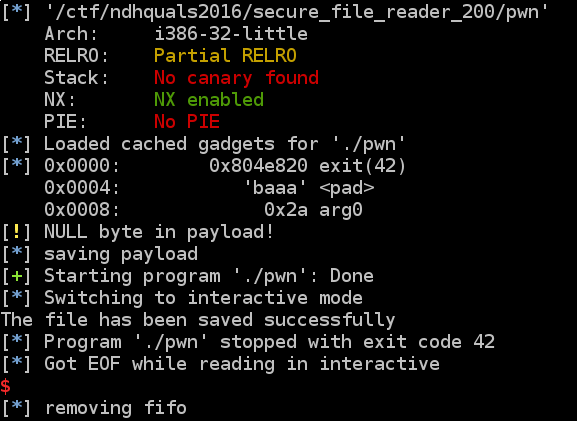
\includegraphics[height=0.7\textheight]{./images/pwntools-exp.png}
  \end{center}
\end{frame}


\begin{frame}
  \begin{center}
    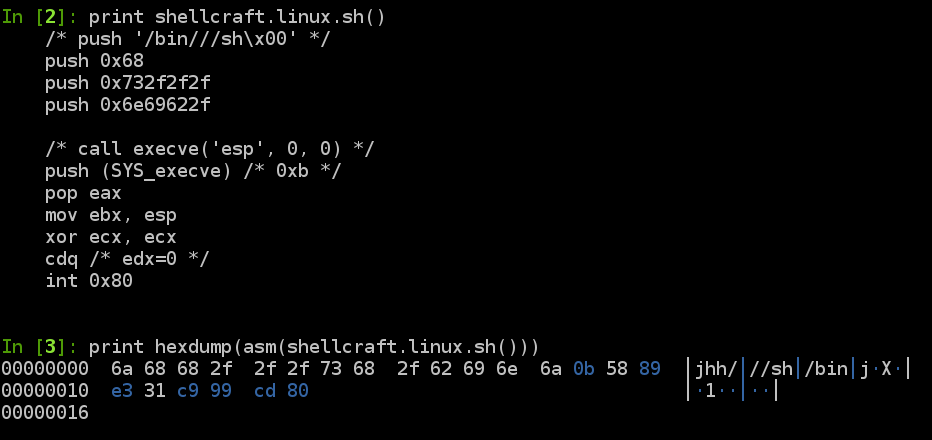
\includegraphics[width=\textwidth]{./images/pwntools-shellcraft.png}
  \end{center}
\end{frame}


\begin{frame}[fragile,allowframebreaks]
  {Binary Decompilers}

  \begin{itemize}
    \item No really good open source binary decompilers \verb+:(+
      %\begin{itemize}
        %\item \href{https://github.com/zneak/fcd}{fcd} gives
      %\end{itemize}
    \item Commercial/Closed-Source
      \begin{itemize}
        \item Hex-Rays/IDA Pro Decompiler (\$\$\$)
        \item \href{http://hopperapp.com/}{Hopper} (\$)
        \item \href{https://retdec.com/}{retdec} (free, webservice, no \verb+x86_64+)
      \end{itemize}
  \end{itemize}
\end{frame}

\begin{frame}[fragile]
  {Bytecode Decompilers}

  \begin{itemize}
    \item Bytecode Decompilers much more sophisticated!
    \item Java/Dalvik bytecode
      \begin{itemize}
        \item intellij built-in decompiler (fernflower)
        \item
          \href{https://bitbucket.org/mstrobel/procyon/}{procyon}
        \item \href{https://github.com/skylot/jadx}{jadx}
        %\item \href{https://github.com/Konloch/bytecode-viewer/}{bytecode
        %viewer}
          \todo[inline]{apktool?}
      \end{itemize}
    \item .net bytecode
      \begin{itemize}
        \item ILSpy, ???
          \todo[inline]{add more?}
      \end{itemize}
  \end{itemize}

\end{frame}


% sagemath - crypto all the things

\begin{frame}
  \todo[inline]{crypto/sage fu. factorization? ecc?}
\end{frame}

% pen & paper - never underestimate



\begin{frame}
  {Learn to Improvise}

  \begin{itemize}
    \item Premature optimization* is the root of all evil!
      \begin{itemize}
        \item * also commenting code
        \item * also clean code
      \end{itemize}
    \item (only true for attack \&\&  \emph{during} CTFs!)
    \item If it works, \ldots it works!
    \item Code-reuse between different CTFs!
  \end{itemize}

\end{frame}

\begin{frame}
	\begin{center}
		\huge A fool with a tool is still a fool!
	\end{center}
\end{frame}

\begin{frame}

  \begin{center}
    {\huge \url{https://hack.more.systems}}
  \end{center}

  \vspace{3em}

  Credits:

  \begin{itemize}
    \item The rest of the Team
    \item \ldots
      \todo[inline]{who?}
  \end{itemize}

\end{frame}
